%!TEX root = <main.tex>
% Chapter 1

\chapter{Introduction} % Chapter title

\label{ch:introduction} % For referencing the chapter elsewhere, use \autoref{ch:introduction} 

%----------------------------------------------------------------------------------------


\section{Contribution}\label{sec:Contribution}


\begin{itemize}
    \item Fast Approximatively Multicut Solvers:

        An approximate solver for the multicut objective, 
        called Cut Clue and Cut (GCG) is proposed (see \ref{ch:multicut} ).
        Experiments show  that CGC is superior w.r.t. 
        runtime compared to state of the art solvers, and find solutions
        very close to global optimal solution (see \ref{ch:multicut_experiments}) 

    \item Generalized Fusion Moves:

        An generalization of fusion moves \cite{lempitsky_2010_pami}


    \item Implemented a Graph library and algorithms within vigra.


\end{itemize}




\section{Some Code stuff}
\begin{lstlisting}[language=python]
>>> from numpy import *
>>> from numpy.fft
\end{lstlisting}
\section{Some Tikz stuff}






\begin{tikzpicture}[scale=0.7,transform shape]
 
  % Draw diagram elements
  \path \practica {1}{Diferencias en componentes electr\'onicos};
  \path (p1.south)+(0.0,-1.0) \practica{2}{Serie de Fourier};
  \path (p2.south)+(-2.5,-1.5) \practica{3}{Antena para HF};
  \path (p3.south)+(0.0,-1.0) \practica{5}{Medidor de SWR};
  \path (p3.south)+(5.0,-1.0) \practica{4}{Amplificador para HF};

  \path (p4.south)+(-2.5,-1.5) \practica{6}{Oscilador de RF};
  \path (p6.south)+(-2.5,-1.25) \practica{7}{Modulador AM};
  \path (p6.south)+(2.5,-1.25) \practica{8}{Demodulador AM};
  \path (p8.east)+(+5.5,0) node (ur1)[ur] {};

  \path (p7.south)+(0.0,-1.5) \practica{9}{Codificador digital};
  \path (p8.south)+(0.0,-1.5) \practica{10}{Decodificador digital};
  \path (p10.east)+(+5.5,0) node (ur2)[ur] {};
  \path (p9.south)+(0.0,-1.5) \practica{11}{Codificador FDM};
  \path (p10.south)+(0.0,-1.5) \practica{12}{Decodificador FDM};
  \path (p12.east)+(+5.5,0) node (ur3)[ur] {};
  \path (p11.south)+(0.0,-1.5) \practica{13}{Codificador SSTV};
  \path (p12.south)+(0.0,-1.5) \practica{14}{Decodificador SSTV};
  \path (p14.east)+(+5.5,0) node (ur4)[ur] {};
  \path (p14.south)+(-2.5,-1.5) \practica{15}{Conmutaci\'on telef\'onica};
  \path (p15.south)+(0.0,-1.0) \practica{16}{Telfon\'ia celular an\'aloga};
  \path (p16.south)+(0.0,-1.5) \practica{17}{Receptor de  telemetr\'ia}; 
  \path (p17.south)+(0.0,-1.5) \practica{18}{Gu\'ias de ondas};
     
  % Draw arrows between elements
  \path [line] (p1.south) -- node [above] {} (p2);

  \path [line] (p2.south) -- +(0.0,-0.5) -- +(-2.5,-0.5)
    -- node [above, midway] {} (p3);
  \path [line] (p3.south) -- node [above] {} (p5) ;
     
  \path [line] (p2.south) -- +(0.0,-0.5) -- +(+2.5,-0.5)
    -- node [above, midway] {} (p4);
  \path [linepart] (p3.east) -- +(+0.5,-0.0) -- +(+0.5,-1.75)
    -- node [left, midway] {} (p4);
  \path [linepart] (p3.east) -- +(+0.5,-0.0) -- +(+0.5,-1.75)
    -- node [left, midway] {} (p4);

  \path [line] (p4.south) -- +(0.0,-0.5) -- +(-2.5,-0.5)
    -- node [above, midway] {} (p6);
  \path [line] (p5.south) -- +(0.0,-0.5) -- +(+2.5,-0.5)
    -- node [above, midway] {} (p6);     
  \path [linepart] (p2.east) -- +(2.75,0.0) -- +(2.75,-5.85)
    -- node [right] {} (p6);
  \path [line] (p6.south) -- +(0.0,-0.25) -- +(-2.5,-0.25)
    -- node [above, midway] {} (p7);
  \path [line] (p6.south) -- +(0.0,-0.25) -- +(+2.5,-0.25)
    -- node [above, midway] {} (p8);
  \path [linepart] (p7.east) -- node [left] {} (p8);
  \transreceptor{p8}{AM banda 40m}{ur1}

  \path [line] (p7.south) -- node [above] {} (p9) ;
  \path [line] (p8.south) -- node [above] {} (p10) ;
  \path [linepart] (p9.east) -- node [left] {} (p10);
  \transreceptor{p10}{CW}{ur2}
  \path [line] (p9.south) -- node [above] {} (p11) ;
  \path [line] (p10.south) -- node [above] {} (p12) ;
  \path [linepart] (p11.east) -- node [left] {} (p12);
  \transreceptor{p12}{FDMDV}{ur3}

  \path [line] (p11.south) -- node [above] {} (p13) ;
  \path [line] (p12.south) -- node [above] {} (p14) ;
  \path [linepart] (p13.east) -- node [left] {} (p14);   
  \transreceptor{p14}{SSTV}{ur4}

  \path [line] (p14.south) -- +(0.0,-0.5) -- +(-2.5,-0.5)
    -- node [above, midway] {} (p15);
  \path [line] (p13.south) -- +(0.0,-0.5) -- +(+2.5,-0.5)
    -- node [above, midway] {} (p15);
  \path [line] (p15.south) -- node [above] {} (p16) ;     
  \path [line] (p16.south) -- node [above] {} (p17) ;
  \path [line] (p17.south) -- node [above] {} (p18) ;
   
  \background{p3}{p1}{p4}{p2}{I}
  \background{p3}{p3}{p4}{p5}{II}
  \background{p3}{p6}{p4}{p7}{III}
  \background{p3}{p9}{p4}{p10}{IV}
  \background{p3}{p11}{p4}{p12}{V}
  \background{p3}{p13}{p4}{p14}{VI}
  \background{p3}{p15}{p4}{p16}{VII}
  \background{p3}{p17}{p4}{p17}{VIII}
  \background{p3}{p18}{p4}{p18}{IX}
\end{tikzpicture}




















\begin{center}
\begin{tabular}{l|ll}
bla & set & vector\\ \hline

denk-450           
& 1.0 & 2.0\\
denk-450 ward         
& 1.0 & 5.0\\

bsd-500           
& 1.0 & 2.0\\
bsd-500 ward         
& 1.0 & 5.0

\end{tabular}
\end{center}



\begin{tikzpicture}[scale=  1,every node/.style={minimum size=1cm},on grid]
        
    %slanting: production of a set of n 'laminae' to be piled up. N=number of grids.
    

    %%%%%%%%%%%%%%%%%%%%%%%%%%%%%%%%%%%%%%%%%%%%%%%%%%%%%%%%%%%%%%%
    % 0 bottom layer
    %%%%%%%%%%%%%%%%%%%%%%%%%%%%%%%%%%%%%%%%%%%%%%%%%%%%%%%%%%%%%%%%
        
    \begin{scope}[
        yshift=0,every node/.append style={
            yslant=0.5,xslant=-1},yslant=0.5,xslant=-1
                     ]
        
        \draw[-latex,thick] (-0.17,2.5) node[right]{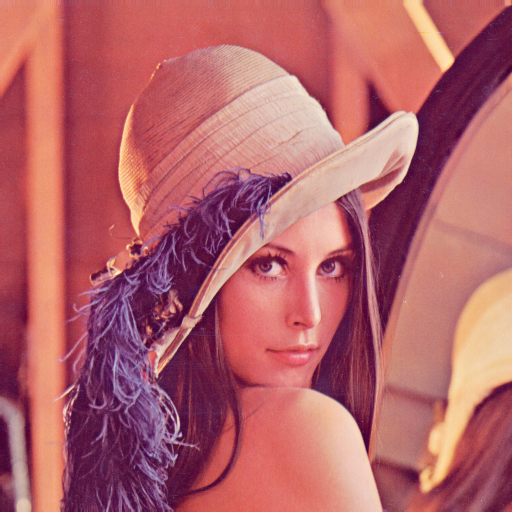
\includegraphics[width=5cm]{fig/lena.png}};
        \fill[white,fill opacity=.0] (0,0) rectangle (5,5);
        \draw[black,very thick] (0,0) rectangle (5,5);
        \draw[step=1.8mm, black] (0,0) grid (5,5);
    \end{scope}

    %%%%%%%%%%%%%%%%%%%%%%%%%%%%%%%%%%%%%%%%%%%%%%%%%%%%%%%%%%%%%%%
    % 1 layer
    %%%%%%%%%%%%%%%%%%%%%%%%%%%%%%%%%%%%%%%%%%%%%%%%%%%%%%%%%%%%%%%%
    
   \begin{scope}[
        yshift=100,every node/.append style={
            yslant=0.5,xslant=-1},yslant=0.5,xslant=-1
                     ]
        
        \draw[-latex,thick] (-0.17,2.5) node[right]{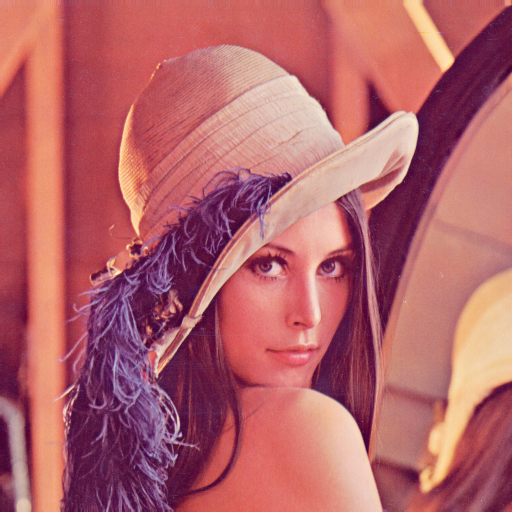
\includegraphics[width=5cm]{fig/lena.png}};
        \fill[white,fill opacity=.0] (0,0) rectangle (5,5);
        \draw[black,very thick] (0,0) rectangle (5,5);
        \draw[step=1.8mm, black] (0,0) grid (5,5);
    \end{scope}
        
     %%%%%%%%%%%%%%%%%%%%%%%%%%%%%%%%%%%%%%%%%%%%%%%%%%%%%%%%%%%%%%%
    % 2 layer
    %%%%%%%%%%%%%%%%%%%%%%%%%%%%%%%%%%%%%%%%%%%%%%%%%%%%%%%%%%%%%%%%
    
   \begin{scope}[
        yshift=200,every node/.append style={
            yslant=0.5,xslant=-1},yslant=0.5,xslant=-1
                     ]
        
        \draw[-latex,thick] (-0.17,2.5) node[right]{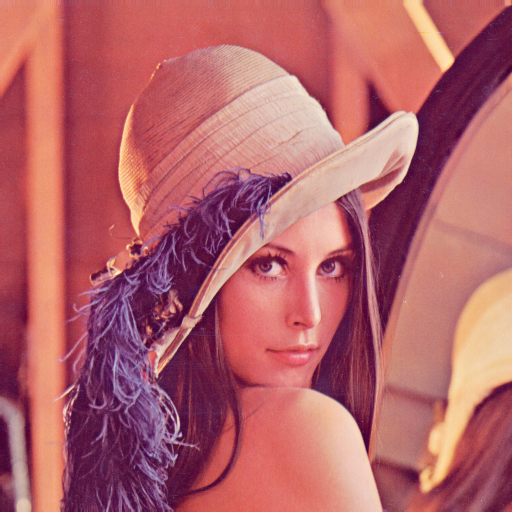
\includegraphics[width=5cm]{fig/lena.png}};
        \fill[white,fill opacity=.0] (0,0) rectangle (5,5);
        \draw[black,very thick] (0,0) rectangle (5,5);
        \draw[step=1.8mm, black] (0,0) grid (5,5);
    \end{scope}
        


    %%%%%%%%%%%%%%%%%%%%%%%%%%%%%%%%%%%%%%%%%%%%%%%%%%%%%%%%%%%%%%%
    % 0 bottom layer
    %%%%%%%%%%%%%%%%%%%%%%%%%%%%%%%%%%%%%%%%%%%%%%%%%%%%%%%%%%%%%%%%
    \draw[-latex,thick] (6.2,2) node[right]{$\mathsf{Grid Graph}$}
         to[out=180,in=90] (4,2);
         
         
         
    %%%%%%%%%%%%%%%%%%%%%%%%%%%%%%%%%%%%%%%%%%%%%%%%%%%%%%%%%%%%%%%
    % 1 layer
    %%%%%%%%%%%%%%%%%%%%%%%%%%%%%%%%%%%%%%%%%%%%%%%%%%%%%%%%%%%%%%%%
    
    \draw[-latex,thick] (6.2,5.5) node[right]{$\mathsf{Region adjacency graph 1}$}
         to[out=180,in=90] (4,5.5);

\end{tikzpicture}






































% We need layers to draw the block diagram
\pgfdeclarelayer{background}
\pgfdeclarelayer{foreground}
\pgfsetlayers{background,main,foreground}

% Define a few styles and constants
\tikzstyle{sensor}=[draw, fill=blue!20, text width=5em, 
    text centered, minimum height=2.5em]
\tikzstyle{ann} = [above, text width=5em]
\tikzstyle{naveqs} = [sensor, text width=6em, fill=red!20, 
    minimum height=12em, rounded corners]
\def\blockdist{2.3}
\def\edgedist{2.5}

\begin{tikzpicture}
    \node (naveq) [naveqs] {Navigation equations};
    % Note the use of \path instead of \node at ... below. 
    \path (naveq.140)+(-\blockdist,0) node (gyros) [sensor] {Gyros};
    \path (naveq.-150)+(-\blockdist,0) node (accel) [sensor] {Accelero-meters};
    
    % Unfortunately we cant use the convenient \path (fromnode) -- (tonode) 
    % syntax here. This is because TikZ draws the path from the node centers
    % and clip the path at the node boundaries. We want horizontal lines, but
    % the sensor and naveq blocks aren't aligned horizontally. Instead we use
    % the line intersection syntax |- to calculate the correct coordinate
    \path [draw, ->] (gyros) -- node [above] {$\vc{\omega}_{ib}^b$} 
        (naveq.west |- gyros) ;
    % We could simply have written (gyros) .. (naveq.140). However, it's
    % best to avoid hard coding coordinates
    \path [draw, ->] (accel) -- node [above] {$\vc{f}^b$} 
        (naveq.west |- accel);
    \node (IMU) [below of=accel] {IMU};
    \path (naveq.south west)+(-0.6,-0.4) node (INS) {INS};
    \draw [->] (naveq.50) -- node [ann] {Velocity } + (\edgedist,0) 
        node[right] {$\vc{v}^l$};
    \draw [->] (naveq.20) -- node [ann] {Attitude} + (\edgedist,0) 
        node[right] { $\mx{R}_l^b$};
    \draw [->] (naveq.-25) -- node [ann] {Horisontal position} + (\edgedist,0)
        node [right] {$\mx{R}_e^l$};
    \draw [->] (naveq.-50) -- node [ann] {Depth} + (\edgedist,0) 
        node[right] {$z$};
    
    % Now it's time to draw the colored IMU and INS rectangles.
    % To draw them behind the blocks we use pgf layers. This way we  
    % can use the above block coordinates to place the backgrounds   
    \begin{pgfonlayer}{background}
        % Compute a few helper coordinates
        \path (gyros.west |- naveq.north)+(-0.5,0.3) node (a) {};
        \path (INS.south -| naveq.east)+(+0.3,-0.2) node (b) {};
        \path[fill=yellow!20,rounded corners, draw=black!50, dashed]
            (a) rectangle (b);
        \path (gyros.north west)+(-0.2,0.2) node (a) {};
        \path (IMU.south -| gyros.east)+(+0.2,-0.2) node (b) {};
        \path[fill=blue!10,rounded corners, draw=black!50, dashed]
            (a) rectangle (b);
    \end{pgfonlayer}
\end{tikzpicture}


















\centering\begin{tikzpicture}[mindmap,scale=0.5, transform shape,
  level 1 concept/.append style={level distance=130,sibling angle=30},
  extra concept/.append style={color=blue!50,text=black}]
  % Applied area: computer science and its subfields

  \begin{scope}[mindmap, concept color=orange, text=white]
    \node [concept] {Informatique}[clockwise from=-5] 
      child {node [concept] (log) {M{\'e}thodes cat{\'e}goriques}}
      child {node [concept] (alg) {Algorithmique}}
      child {node [concept] (cod) {Compression \& transmission}}
      child {node [concept] (img) {Tra{\^i}tement des images}}
      child {node [concept] (opt) {Optimisation}}
      child {node [concept] (res) {R{\'e}seaux}};
  \end{scope}

  % Applied area: theoretical physics and its subfields

  \begin{scope}[mindmap, concept color=red,text=white]
    \node [concept] at (-5,-15) {Physique}
      child [grow=-10, level distance=160]
        {node [concept] (qin) {Calcul quantique}}
      child [grow=20] 
        {node [concept] (csm) {Astronomie \& cosmologie}}
      child [grow=110] 
        {node [concept] (mat) {Mati{\`e}re condens{\'e}e}};
  \end{scope}

  % Applied area: biology and its subfields

  \begin{scope}[mindmap, concept color=green!50!black,text=white]
    \node [concept] at (6.5,-15) {Biologie} 
      child [grow=165, level distance=120] 
        {node [concept] (med) {M{\'e}decine}}
      child [grow=60] 
        {node [concept] (gen) {G{\'e}nomique}};
  \end{scope}

  % Applied area: economics (one subfield)

  \begin{scope}[mindmap, concept color=violet, text=white]
    \node [concept] at (11,-14) {{\'E}conomie}
      child [grow=70, level distance=120] 
        {node [concept] (dec) {Choix \& prise de d{\'e}cision}};
  \end{scope}

  % Researchers listed by their main specialization in mathematics

  \begin{scope}[mindmap, concept color=blue]

    % Combinatorics and discrete mathematics 
    \node [concept, text=white] at (5.2,-10.8) 
      {Combinatoire \& math{\'e}matiques discr{\`e}tes} 
      [clockwise from=150]
      child [concept color=blue!50] {node [concept] (ver) {Vereschagin}}
      child [concept color=blue!50, level distance=125] 
        {node [concept] (kab) {Kabatyanski, Tsfasman, Rybakov, Zykin}}
      child [concept color=blue!50] 
        {node [concept] (kch) {Kucherov, Roytberg}}
      child [concept color=blue!50] {node [concept] (raf) {Raffinot}}
      child [concept color=blue!50, level distance=135]
        {node [concept] (ksh) {Koshevoy}};

    % Partial differential equations
    \node [concept, text=white] at (-3,-11) 
      {Equations aux d{\'e}riv{\'e}es partielles 
        \& m{\'e}thodes num{\'e}riques}
      child [concept color=blue!50, grow=0, level distance=140] 
        {node [concept] (lhc) {Loh{\'e}ac}}
      child [concept color=blue!50, grow=60, level distance=115] 
        {node [concept] (otr) {OTARIE (Sobolevski)}}
      child [concept color=blue!50, grow=95] {node [concept] (ndr) 
        {Nadirashvili}};

    % Probability
    \node [concept, text=white] at (-7.2,-3.2) {Probabilit{\'e}s}
      child [concept color=blue!50, grow=-70, level distance=120] 
        {node [concept] (rbk) {Rybko}};

    % Logic
    \node [concept, text=white] at (11.5,-5) {Logique}
      child [concept color=blue!50, grow=165, level distance=120] 
        {node [concept] (sht) {Shehtman}};
  \end{scope}

  % Connections of researchers to applied subfields

  \begin{pgfonlayer}{background}
    \draw [circle connection bar]
      (kab) edge (cod)
      (kch) edge (alg) edge (gen)
      (lhc) edge (med)
      (ksh) edge (dec)
      (ndr) edge (mat)
      (otr) edge (opt) edge (csm) edge (img)
      (raf) edge (alg) edge (gen)
      (rbk) edge (res) edge (mat)
      (sht) edge (log) edge (dec)
      (ver) edge (qin) edge (cod);
  \end{pgfonlayer}

\end{tikzpicture}


\newpage





% Below we mix an ordinary equation with TikZ nodes. Note that we have to
% adjust the baseline of the nodes to get proper alignment with the rest of
% the equation.
\begin{equation}
\omega_{e} = 
        \tikz[baseline]{\node[fill=blue!20,anchor=base] (te)        
            {$ f_{\epsilon}(X_{e}) $};
        } +
        \tikz[baseline]{\node[fill=red!20,anchor=base] (tuv)
            {$  d_{\nu}(X_u,X_v) $};
        } +   
        \tikz[baseline]{ \node[fill=green!20,anchor=base] (tr)
            {$r(|u|,|v|,|e|)$};  
        }
\end{equation}

\begin{itemize}
    \item Edge indicator:          \tikz\node [fill=blue!20,draw,circle] (ne) {};
        \begin{itemize}
         \item Gradient magnitude
         \item Eigenvalues of hessian
        \end{itemize}
    \item Node feature difference: \tikz\node [fill=red!20,draw,circle] (nuv) {};
       \begin{itemize}
         \item L1,L2
         \item Histogram differences ($\chi^2$,Earth movers distance)
       \end{itemize}
    \item Geometric regularizer:   \tikz\node [fill=green!20,draw,circle] (nr) {};
       \begin{itemize}
         \item Wards criterion \cite{ward_clustering}
         \item Log Ward criterion
         \item None 
      \end{itemize}
\end{itemize}

% Now it's time to draw some edges between the global nodes. Note that we
% have to apply the 'overlay' style.
%\begin{tikzpicture}[overlay]
%        \path[->] (ne) edge [bend right] (te);
%        \path[->] (nuv) edge [bend right] (tuv);
%        \path[->] (nr) edge [out=0, in=-90] (tr);
%\end{tikzpicture}



% -------------------------------------------------
% Set up a new layer for the debugging marks, and make sure it is on
% top
\pgfdeclarelayer{marx}
\pgfsetlayers{main,marx}
% A macro for marking coordinates (specific to the coordinate naming
% scheme used here). Swap the following 2 definitions to deactivate
% marks.
\providecommand{\cmark}[2][]{%
  \begin{pgfonlayer}{marx}
    \node [nmark] at (c#2#1) {#2};
  \end{pgfonlayer}{marx}
  } 
\providecommand{\cmark}[2][]{\relax} 


